\chapter{Solução Proposta: \textit{Clean Pool Robot}}
\section{Visão Global}
O \textit{Clean Pool Robot} é um robô de aspiração de fundos de piscinas. O
mecanismo do mesmo será composto por dois métodos para que o fundo da piscina
possa ser aspirado: o primeiro baseia-se na escovação do chão e o segundo a
sucção das impurezas desprendidas do piso da piscina.
\par
O primeiro método tem foco nas escovas que estão situadas na parte inferior
do robô. As escovas realizam movimentos giratórios fazendo com que suas cerdas
entrem em contato com o chão retirando  impurezas, como por exemplo: algas e
grãos de terra.
\par
Após a escovação, é realizado outro método, a sucção das impurezas desprendidas
do piso da piscina  além de outras impurezas que estiverem próximas à área de
atuação do robô, por exemplo: pequenos ramos e folhas. Por meio de uma bomba, a
água é sugada por uma abertura situada na parte inferior e passa por um saco onde
as partículas de maiores dimensões ficam depositadas. Depois de passar pelo saco,
a água passa por um filtro removível. As impurezas menores ficam retidas no filtro.
Por meio de um sistema de expulsão de água, esta sairá a uma velocidade muito superior
à velocidade de entrada no início do processo, ajudando também na movimentação do robô.
\par
Com o término da limpeza na piscina, haverá a necessidade dos filtros serem limpos
para retirada das impurezas colhidas na aspiração da água. Assim, após cada utilização
o usuário deverá limpar os filtros internos do \textit{Clean Pool Robot}.
\par
O produto desenvolvido será responsável apenas pela retirada da sujeira decantada
no fundo da piscina, ou seja, o \textit{Clean Pool Robot} não limpará as paredes
ou superfície da piscina. Além disso, as piscinas ideais para a operação do Robot
são as retangulares, sem inclinações e azulejadas. É ideal também que o robô seja
lançado na piscina no meio da largura maior, evitando que o fio fique totalmente
esticado quando o robô estiver na quina oposta do lançamento.
\par
Como diferencial, o \textit{Clean Pool Robot} será um produto nacional com custo
mais acessível e que possui percurso não aleatório.
\par
O \textit{Clean Pool Robot} pode ser dividido em duas grandes partes, uma compondo a
estrutura (apelidada de corpo) e o outro a parte lógica (apelidada de mente) do
robô. Cada uma dessas será explicada posteriormente.

\section{Percurso do Robô}
O esquemático abaixo mostra uma ideia inicial de como o robô percorrerá a piscina
a ser limpada.
\par
\begin{figure}[h]
    \centering
    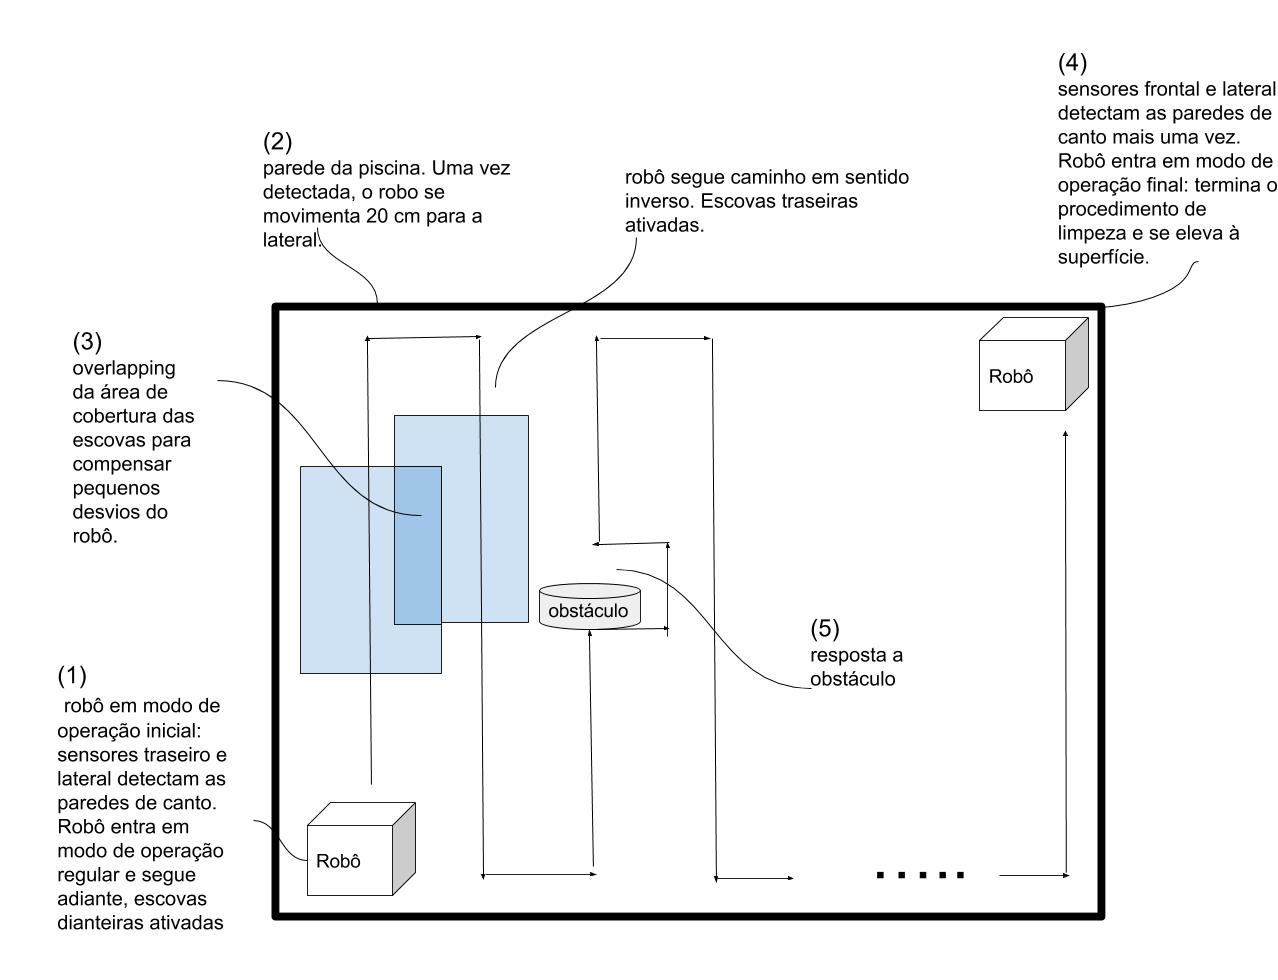
\includegraphics[width=\textwidth]{figures/schema-way-robot.jpg}
    \caption{Demonstrativo do percurso de limpeza do robô.}
    \label{fig:schema-way-robot}
  \end{figure}
\par
O robô limpador foi projetado para ser capaz de percorrer toda a área da superfície
inferior de piscinas retangulares e sem inclinação. A varredura é feita de forma
totalmente autônoma pelo sistema, com a \textit{Raspberry pi} como unidade central de
controle de todos elementos periféricos: sensores de distância, servo motores,
sensores de pressão, etc. É necessário o usuário apenas posicionar o limpador em
uma das bordas da piscina e recolhê-lo quando o processo de limpeza estiver completo.
\par
Com o intuito de simplificar o sistema, optou-se por permitir ao robô mover-se apenas
em duas direções, horizontal e vertical, em ambos os sentidos. Desta forma,
baseando-se em projetos similares como o descrito na patente \textit{POOL CLEANER
DIRECTIONAL CONTROL METHOD AND APPARATUS} (2001, patent No:US 6,299,699 B1), o
padrão ideal de varredura consiste em uma sequência de travessias longitudinais
paralelas, partindo de uma borda da piscina à outra, como pode ser visto na figura
acima.
\par
O limpador inicia o processo de varredura assim que os sensores de distância,
localizados em cada uma das laterais do robô, detectam que ele se encontra em
uma das quinas da piscina (1).  O limpador segue em linha reta em direção à
próxima parede, com os motores das escovas ativados para fazer a limpeza do chão.
Uma vez próximo à parede, limpador então desloca-se para a direita cerca de 20
centímetros e segue o percurso em linha reta, em sentido contrário (2). O deslocamento
de 20 centímetros é tal que haja uma sobreposição das áreas varridas pelas escovas
em ambos os sentidos percorridos (3), de forma a compensar qualquer desvio de
rota não detectado pelo giroscópio. O limpador retorna à parede inicial, desloca-se
outros 20 centímetros para a direita  e segue mais uma vez em sentido oposto. Este
procedimento se repete até que o robô chegue à parede direita da piscina (4). Na
eventualidade de o robô se encontrar, no meio do percurso,  com um obstáculo grande
o bastante para ser detectado pelos sensores de distância, o limpador deverá desviar
do obstáculo e seguir sua rota original (5).

\section{Modos de Operação}
A movimentação do robô limpador é definida por quatro modos de operação distintos,
referentes às quatro etapas de funcionamento: inicial, operação regular,
resposta a obstáculo e final.
\par
Na etapa inicial, o limpador deve ser capaz de submergir ao fundo da piscina e
posicionar-se em um dos quatro vértices. Uma vez posicionado ele inicia o modo
de operação regular e realiza o percurso de limpeza  explicado anteriormente.
Terminado o percurso, o robô deve ser capaz de “emergir” à superfície para ser
coletado pelo usuário. Caso o limpador se depare com um obstáculo de grande porte
em seu percurso, ele deve ser capaz de circundar o obstáculo e retornar ao modo de
operação regular.

\subsection{Modo de Operação Regular}
O fluxograma a seguir define com mais detalhes as lógicas de funcionamento
do robô limpador para o modo de operação regular, levando em conta todos os
componentes eletrônicos envolvidos.
\par
\begin{figure}[h]
  \centering
  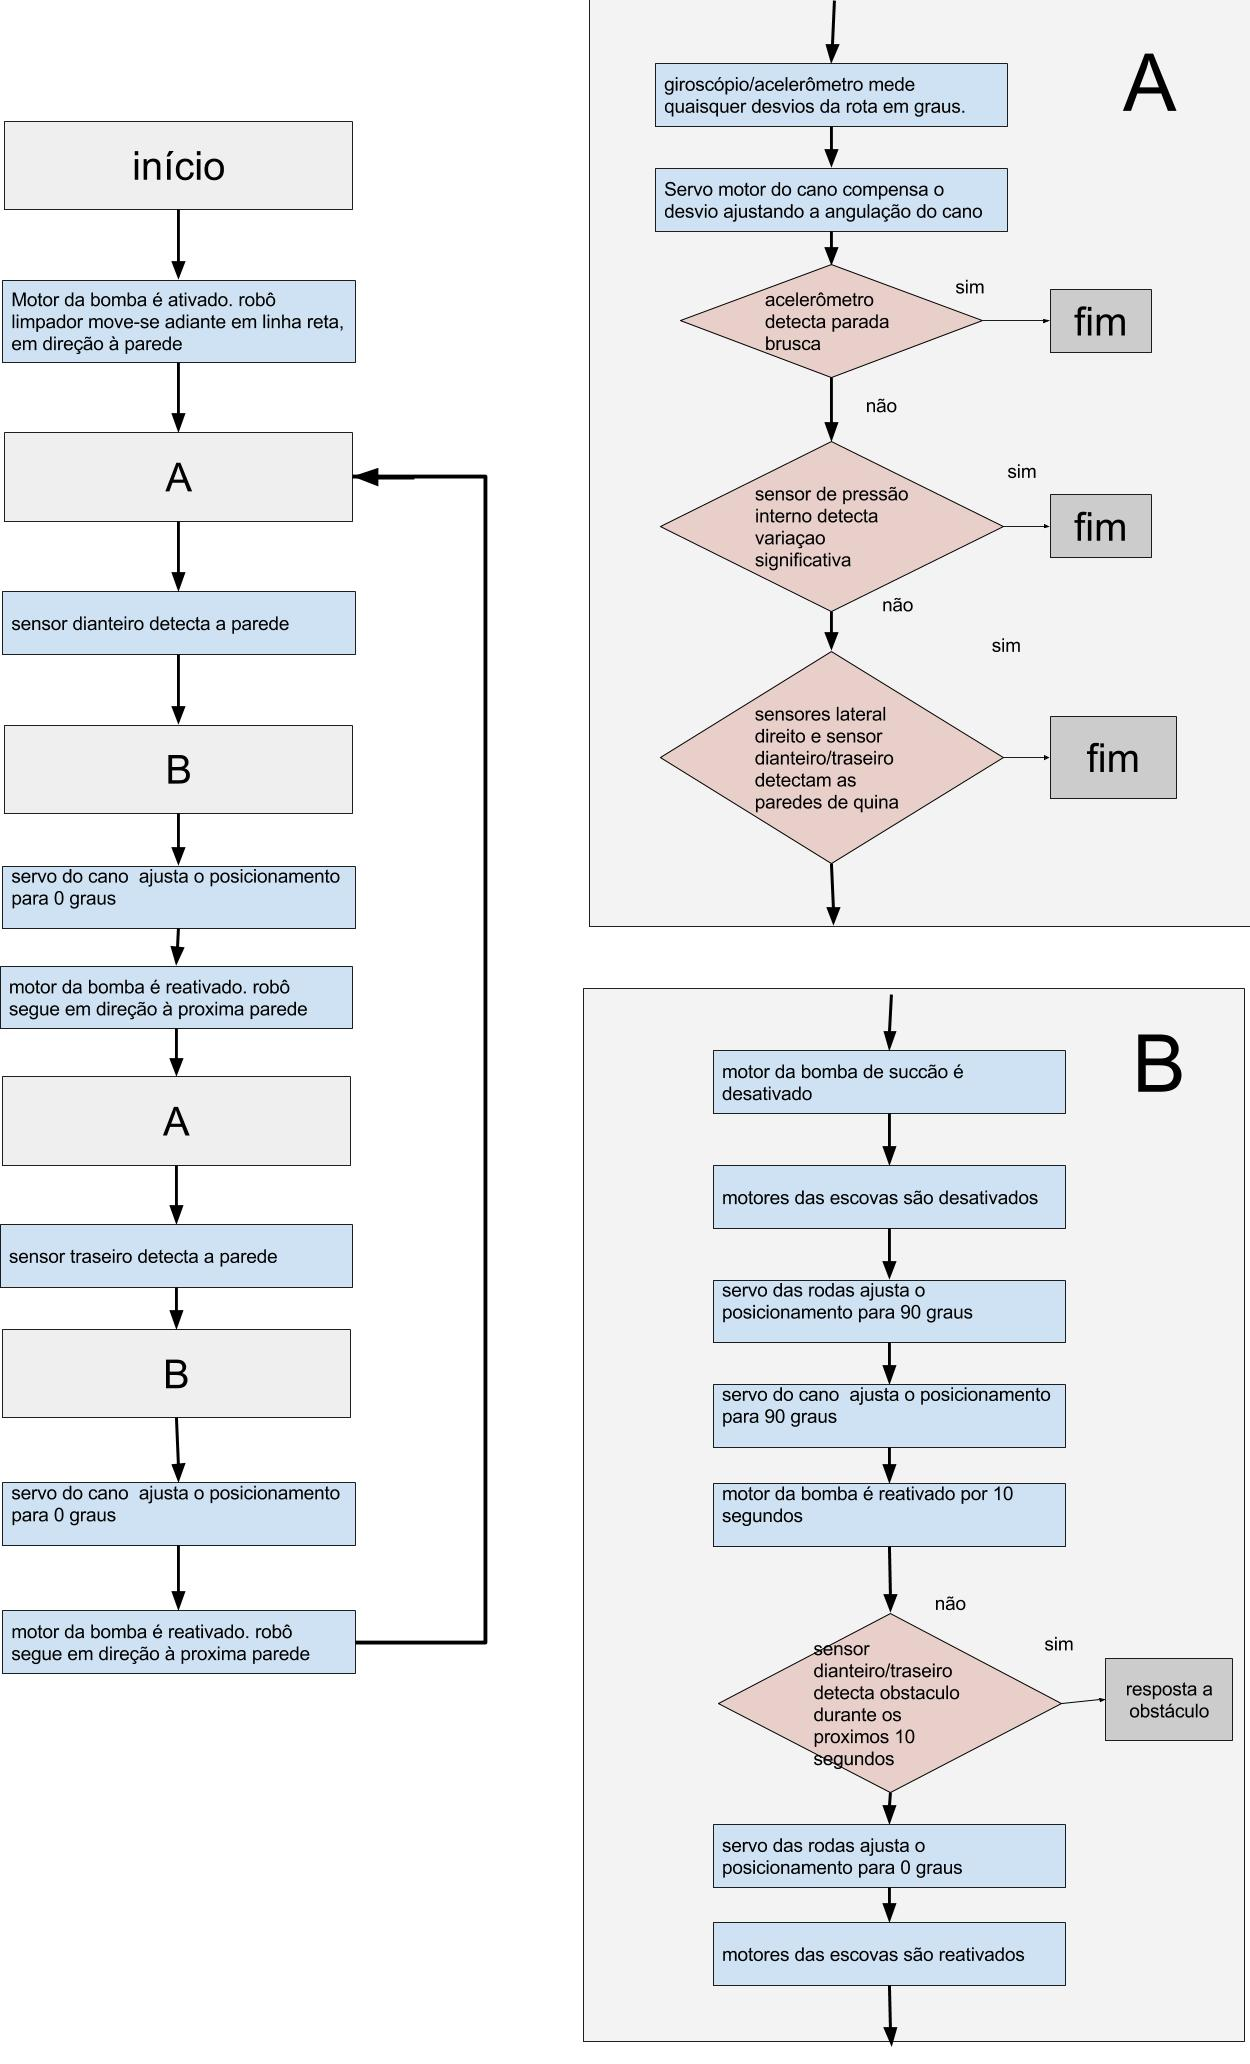
\includegraphics[width=0.9\textwidth]{figures/flow-regular-robot.jpg}
  \caption{Modo de Operação Regular do \textit{Clean Pool Robot}}
  \label{fig:flow-regular-robot}
\end{figure}
\FloatBarrier

\subsection{Resposta a Obstáculos}
Foram definidos três casos de obstáculo que o robô poderá encontrar em seu percurso.

\begin{description}
\item[Caso 1:] \textit{Obstáculo pequeno capaz de ser sugado pela bomba e obstruir os
filtros do limpador}. Neste caso, o sensor de pressão interna detecta qualquer
variação de pressão na caixa do filtro.  A operação de limpeza é então abortada
e o robô para e se “eleva à superfície” (modo de operação final).
\item[Caso 2:] \textit{Obstáculo grande não detectado pelos sensores, resultando em
colisão direta com obstáculo}. Neste caso, o acelerômetro detecta parada brusca
do robô. A operação de limpeza é  também abortada e o robô para e se” eleva à
superfície” (modo de operação final).
\item[Caso 3:] \textit{Obstáculo grande e detectável pelos sensores de distância}. O
robô não é capaz de imediatamente discernir a parede da piscina com o obstáculo
e segue, a princípio, com seu procedimento como se o obstáculo fosse de fato parede.
\end{description}
\par
O fluxograma a seguir detalha em alto nível de abstração as etapas que o sistema
de controle devem seguir para circundar o obstáculo neste caso
\par
\begin{figure}[h]
  \centering
  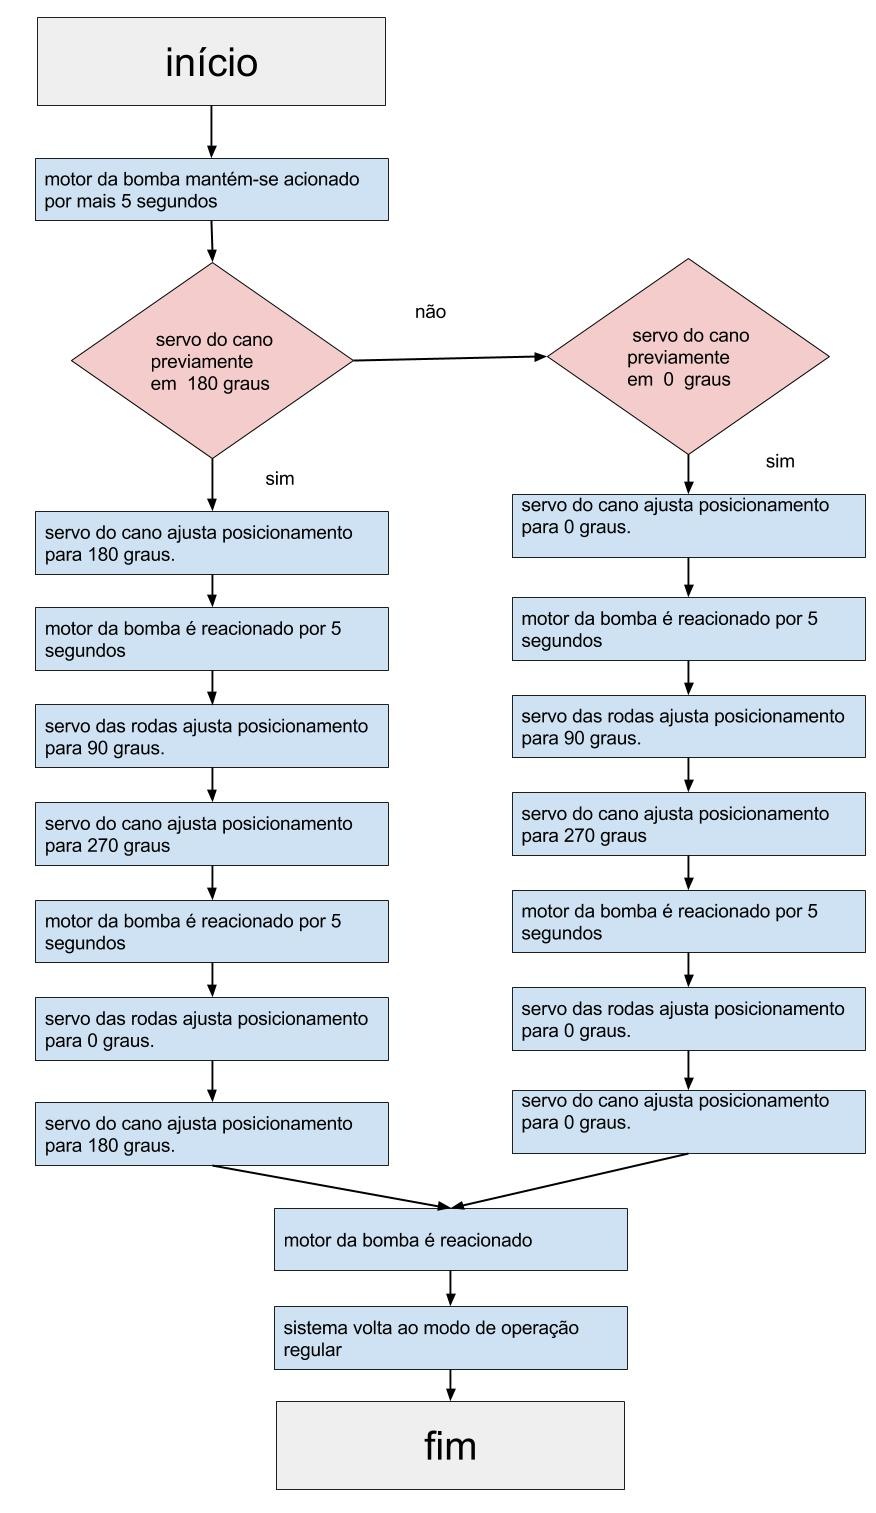
\includegraphics[width=0.9\textwidth]{figures/flow-robot-obstacle.jpg}
  \caption{Modo de Operação Resposta a Obstáculos do \textit{Clean Pool Robot}}
  \label{fig:flow-obstacle-robot}
\end{figure}
\FloatBarrier

\subsection{Modo de Operação Inicial e Final}
Antes de começar a varredura da piscina, o robô deve primeiro posicionar-se
perfeitamente em um dos 4 cantos da piscina. O fluxograma a seguir detalha
as etapas do processo a partir do momento em que o limpador chega ao fundo
da piscina.
\par
\begin{figure}[h]
  \centering
  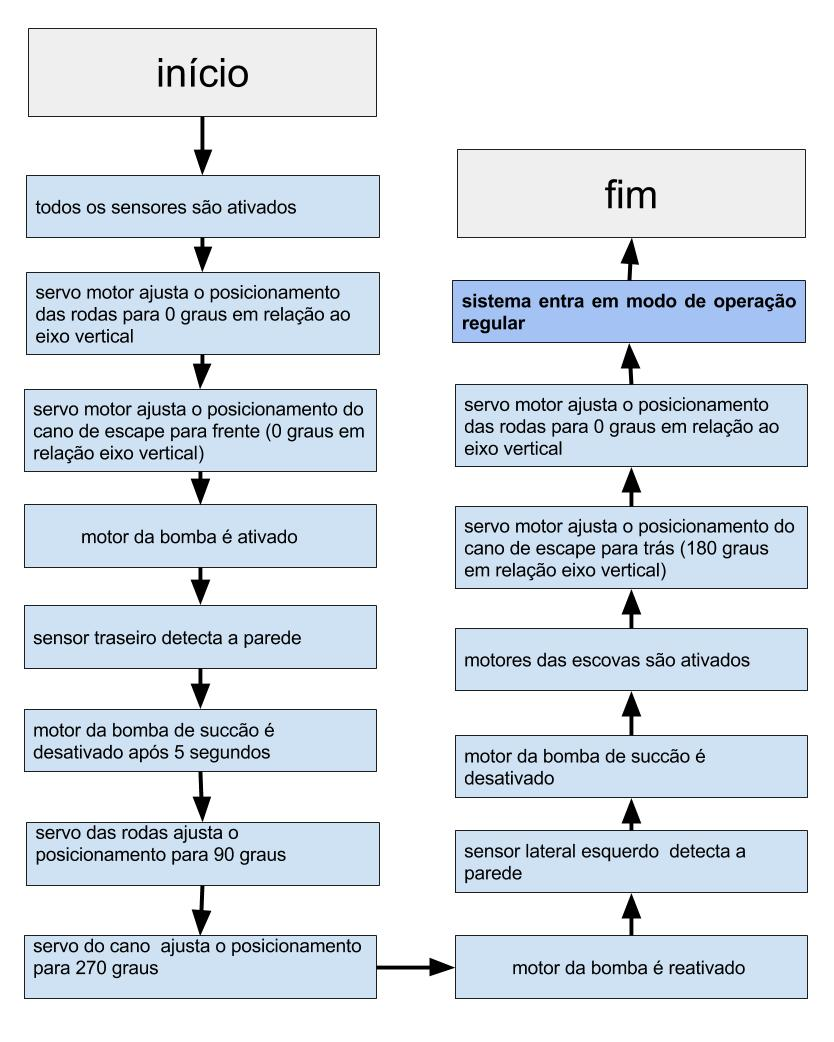
\includegraphics[width=0.9\textwidth]{figures/flow-initial-robot.jpg}
  \caption{Modo de Operação Inicial e Final do \textit{Clean Pool Robot}}
  \label{fig:flow-initial-robot}
\end{figure}
\FloatBarrier

\section{O Corpo do Robô (Aeroespacial, Automotiva e Energia)}
A figura abaixo mostra a primeira modelagem do\textit{Clean Pool Robot}. O modelo
apresenta uma bomba de sucção (1), uma caixa com os filtros para as impurezas
(2), dois motores para a rotação das escovas (3), uma saída superior da água
filtrada (4), quatro rodas próprias para rolagem em ambientes aquáticos (5),
dois enrolamentos com escovas para soltura da sujeira do piso da piscina (6),
duas entradas para sucção da água e impurezas do fundo da piscina (7), uma
entrada da fonte de alimentação externa (8) e uma caixa com os circuitos
eletrônicos do robô (9). Abaixo da figura estão detalhados as especificações
de cada componente utilizado no Robô.
\par
\begin{figure}[h]
  \centering
  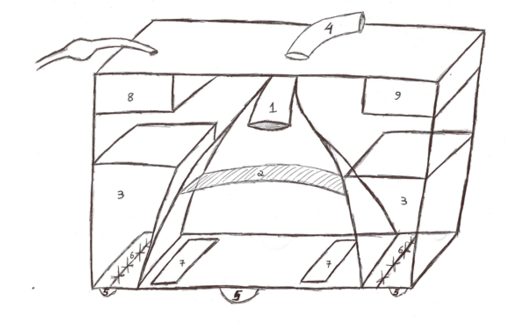
\includegraphics[width=0.9\textwidth]{figures/croqui.png}
  \caption{ Croqui inicial do \textit{Clean Pool Robot}}
  \label{fig:initial_croqui}
\end{figure}
\FloatBarrier
\par
Por motivo de resistência ao movimento o formato do robô foi modificado para
melhor aproveitamento das forças aerodinâmica envolvidas, as alterações no
desenho inicial foram feitas com a intenção de diminuir a força de arrasto, a
estrutura conta agora com cantos e arestas arredondadas conforme a Figura.
\par
\begin{figure}[h]
  \centering
  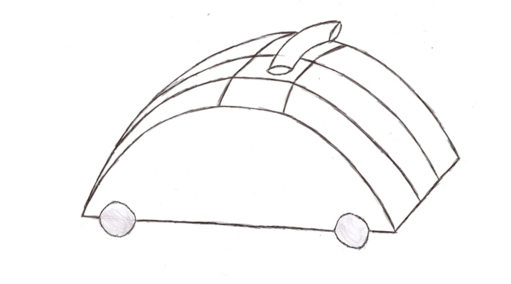
\includegraphics[width=0.9\textwidth]{figures/better-croqui.png}
  \caption{ Croqui melhorado do \textit{Clean Pool Robot}}
  \label{fig:better-croqui}
\end{figure}
\FloatBarrier
\par
\begin{description}
\item[Bomba:] O processo de aspiração da piscina feito pelo robô será uma das
principais tarefas executadas pela bomba de sucção, bem como também o processo
de movimentação do robô embaixo d’água. Para isso, é importante que a bomba
seja resumidamente forte o suficiente para sugar e gerar movimentação por meio
do fluxo de saída da bomba. A sucção será conectada diretamente ao reservatório
onde acontecerá a filtragem da água. Com isso, é esperado que a vazão diminua
entorno de 30 a 40\% da sua vazão nominal de saída. É importante ressaltar que
as únicas funções da bomba neste projeto são apenas filtrar e movimentar por empuxo.
\par
A análise do dimensionamento adequado para a bomba será feito a partir de sua vazão
nominal. Para isto, tem-se por especificações primárias bombas que ofereçam vazões
altas e que trabalhem em uma profundidade máxima de 3 metros. 
\par
Após o cálculo de sua velocidade de saída utilizando a sua vazão e área de jato,
serão calculados o empuxo desenvolvido e sua respectiva pressão de saída. É importante
salientar que a pressão de saída deverá ser sempre positiva e superior a pressão
hidrostática a qual está submetido o bocal de propulsão.
\par
Ao longo de alguns estudos, observou-se que para o problema dado os modelos de bombas
que melhor se enquadram são as moto bombas, uma vez que as mesmas possuem baixo peso e
altas velocidades de saída, bem como altas vazões.
\par
O modelo parcialmente proposto será uma bomba do tipo Bilge , na qual tem as seguintes
características:
  \begin{itemize}
  \item Peso: aproximadamente 3 kg;
  \item Modelo: 500 GPH - com Tensão de trabalho 12 V DC - Amperagem de 1.9;
  \item Formato: Cilíndrico alterável;
  \item Área de operação entorno de até 3,7 metros.
  \end{itemize}
\par
\begin{figure}[h]
  \centering
  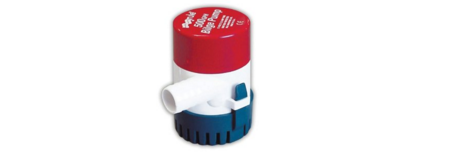
\includegraphics[width=0.9\textwidth]{figures/waterbomb.png}
  \caption{ Bomba proposta}
  \label{fig:waterbomb}
\end{figure}
\FloatBarrier
\par
\textit{Dimensionamento do Teste:} Diante de todo processo de dimensionamento
e a propulsão do robô abaixo d’água, foi pensado em um teste para analisar se
há coerência nos cálculos realizados. Sendo assim, o teste irá ser realizado
com um uma estrutura móvel e uma bomba de aquário. É esperado, com isso, validar
os cálculos realizados no que tange a movimentação da estrutura. Para isso,
foram explicados por meio dos métodos de cálculos descritos a seguir. Segundo
ISE(2000), quando um veículo submersível se movimenta com velocidade constante,
a propulsão gerada pelos propulsores se iguala à força de arrasto produzida. A
força de arrasto será obtida a partir da soma da força de arrasto devido a 
movimentação do veículo mais a força de arrasto devido o cabo de alimentação.
\begin{displaymath}
  Fp = Fa = Fv + Fc = \frac{1}{2}\rho V^{2}_{v}Cd_{v} + \frac{1}{2}\rho V^{2}_{c}Cd_{c}
\end{displaymath}
Onde $Fp$ e $Fa$ referem-se à força de propulsora e força de arrasto total
respectivamente, $Fv$ e $Fc$ são as forças de arrasto devido ao veiculo e ao cabo de
alimentação, $\rho$ é a densidade do fluido, $V_{v}$ e $V_{c}$ velocidades do
veículo e do cabo e por fim, $Cd_{v}$ e $Cd_{c}$ representam os coeficientes
de arrasto.
\par
A potência necessária para a bomba pode ser obtida em função da força propulsiva
e da velocidade do veiculo.
\begin{displaymath}
  P = Fp\frac{d}{t}
\end{displaymath}
Onde $d$ é a distancia percorrida, $t$ o tempo e $P$ a potência desejada.
\par
Os coeficientes de arrasto são medidos experimentalmente, para fluidos como
ar podem ser encontrados tabelados em função da velocidade do veiculo em relação
à velocidade do som nas condições do ambiente em questão (número de \textit{Mach}), uma
vez que este pode sofrer alterações devido a temperatura envolvida, meio de
propagação etc. Quando o veículo estudado se movimento em fluido líquido como a
água por exemplo, o coeficiente de arrasto deve ser medido em função do número
de Reynolds, (Eng et al., 2008) que por sua vez é calculado pela equação abaixo.
\begin{displaymath}
  Re = \frac{VD}{\upsilon}
\end{displaymath}
Onde $V$ equivale a velocidade do veículo, $D$ o diâmetro e $\upsilon$ a viscosidade
cinemática do fluido.
\par
\begin{figure}[h]
  \centering
  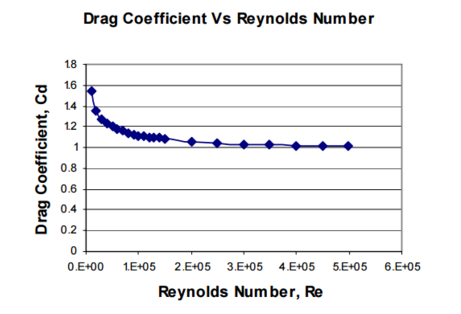
\includegraphics[width=0.9\textwidth]{figures/graphic-reynolds.png}
  \caption{Coeficiente de arrasto em função do numero de Reynolds}
  \label{fig:graphic-reynolds}
\end{figure}
\FloatBarrier
\par
Inicialmente a bomba utilizada será uma bomba de aquário, o que servirá de
parâmetro para a determinação da bomba correta. Para isso, serão realizados
testes com essa bomba para comprovação dos cálculos descritos acima.

\item[Sistema Filtrador:]
\end{description}